\chapter{Introduction to Maritime Surveillance and Trajectory Prediction}

This chapter introduces the core problem addressed by this project: the need for an advanced, AI-driven maritime surveillance system. It provides an overview of the topic, details the primary motivation and objectives, reviews existing literature briefly, and outlines the overall organization of the report.

\section{Introduction}
International trade depends heavily on global waterways. Managing the vast number of commercial, naval, and private vessels operating at any given moment demands accurate and scalable surveillance systems. Traditionally, maritime authorities have turned to tools like radar, the \gls{ais}, and manual visual monitoring to keep track of ship traffic. Figure~\ref{fig:universe} shows a typical \gls{ais} interface often found in coastal control rooms.

While these conventional systems work reasonably well under controlled conditions, they increasingly struggle to handle the sheer volume of modern maritime operations. Radar gives reliable location coordinates but falls short of providing the visual context needed to classify different types of vessels. On the other hand, \gls{ais} is rich in vessel-specific information but completely relies on voluntary signal transmission. This makes it essentially useless for tracking non-cooperative ships or those engaged in illegal activities. Relying on manual video surveillance provides the necessary visual confirmation, but it faces serious scalability issues; human operators suffer from fatigue when trying to monitor multiple camera feeds simultaneously. More importantly, these older methods share a common flaw: they are fundamentally reactive. They only alert authorities when an event is already unfolding, rather than predicting it beforehand.

The rapid progression of deep learning technologies presents a practical avenue to shift from reactive monitoring to proactive forecasting. By merging convolutional neural networks designed for object detection with sophisticated appearance-based trackers and recurrent neural networks for temporal analysis, it is now possible to build systems that automatically find, track, and predict where vessels are heading. This work focuses on constructing an end-to-end pipeline to accomplish exactly that. Ultimately, such an approach supports the United Nations \glspl{sdg} 9 (Industry, Innovation and Infrastructure) and \gls{sdg} 14 (Life Below Water) by enabling safer coastal environments and actively protecting marine ecosystems. Furthermore, transitioning away from heavily manual surveillance processes dramatically reduces operational overhead for coastal authorities. A streamlined, AI-assisted monitoring framework allows port operators to focus their attention primarily on critical alerts and verified anomalies rather than passively watching countless hours of benign maritime traffic. This technological paradigm shift ultimately paves the way for smarter, more responsive global port management.

\begin{figure}[H]
\centering
	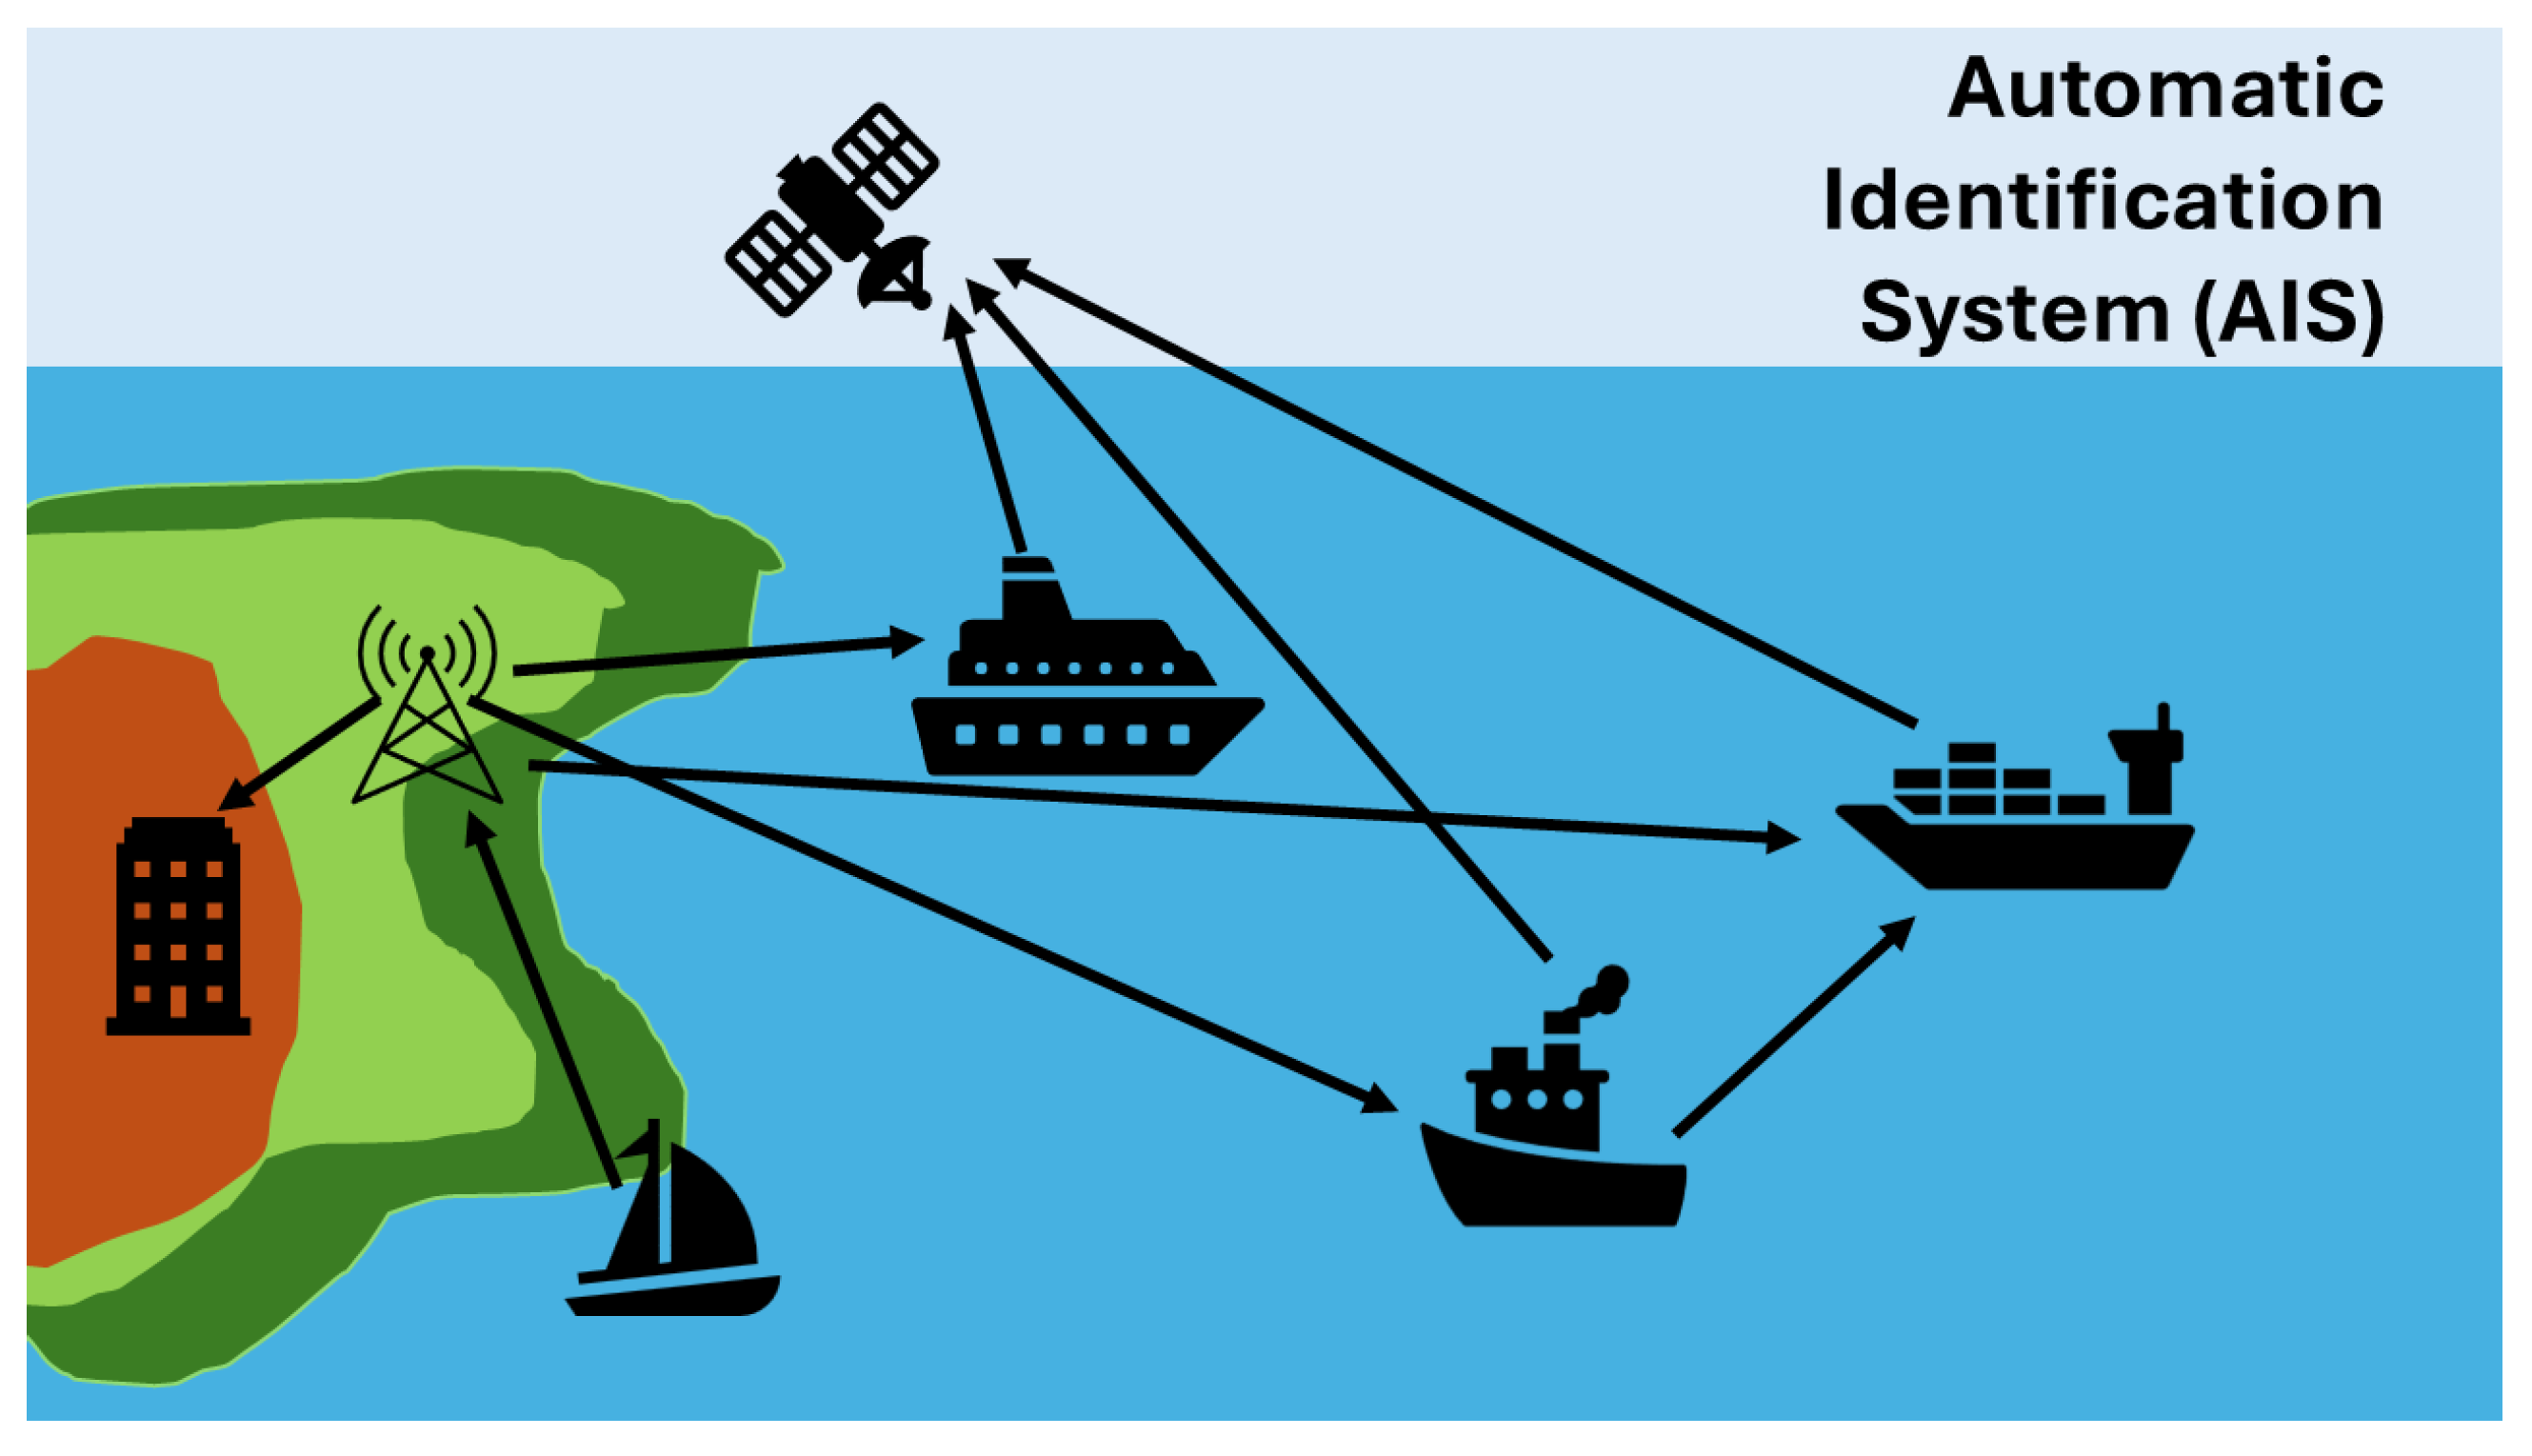
\includegraphics[scale=1]{Chapter1/Figures/ais.jpeg}	
	\caption{\glsentryshort{ais} System used in Maritime Surveillance}
	\label{fig:universe}
\end{figure}

\section{Motivation}
Currently, port authorities and coastal security teams rely on infrastructure that was never designed for the density of today's maritime traffic. Without the ability to reliably cross-reference live visual feeds with \gls{ais} logs, issues like unauthorized border crossings, smuggling, and illegal fishing continue largely unchecked. Solving this problem technically is far from trivial. It demands localizing vessels accurately and keeping track of their unique identities even when they are temporarily hidden by obstacles. Furthermore, predicting their future paths under ever-changing environmental conditions adds another layer of complexity.

Beyond the purely technical aspects, the real-world consequences of poor surveillance, ranging from frequent maritime collisions to severe damage to marine biodiversity, provided the core motivation for this research. Building an automated, vision-driven tool to forecast vessel paths is a direct response to these pressing operational challenges.

\section{Literature Review}
The push towards intelligent maritime surveillance has sparked a considerable amount of research recently. Although Chapter 2 delves deeply into this existing body of work, this section offers a brief overview to highlight the gaps that our project targets.

Much of the current literature treats the tasks of detecting and tracking ships as entirely separate problems. For detection, lightweight models like EGM-\gls{yolov8} have shown they can lower computational costs while keeping recall rates high \parencite{Li2024, Li2025}. Additionally, fine-tuning \gls{yolov8} on maritime-specific datasets has demonstrated that models can effectively manage difficult sea conditions and diverse ship orientations \parencite{Jian2024, Jian2025}. To combat adverse weather, networks like RT-FogNet have been developed to ensure detection remains stable even when hampered by heavy fog or intense surface glare \parencite{Yuan2024, Yuan2026}.

However, simply finding a ship in a single video frame only solves half the problem. Tracking these identified vessels across a dynamic environment introduces persistent challenges such as identity switching and occlusion. Some researchers have tried to address this by combining YOLOv7-tiny with StrongSORT \parencite{Hao2025}, while others have augmented DeepSORT with Optical Character Recognition (OCR) to read hull numbers directly \parencite{Ma2024, Ma2026}. While studies by \cite{Zhang2024Survey} and \cite{Zhang2025} rightly point out that scale variations and visual occlusions are the biggest hurdles in tracking, the workarounds often fall short in practice. Relying on OCR, for instance, breaks down almost immediately when visibility drops or vessels are too far away.

Perhaps the most glaring omission in current research is the lack of cohesive systems that also predict future movement. Most proposed pipelines either detect without tracking properly, or track without attempting to forecast where the ship is going next \parencite{Hao2025, Zhang2025, Li2025, Jian2025, Ma2026, Yuan2026}. Our project tackles this gap head-on by bringing together \gls{yolov8} for detection, \gls{deepocsort} for appearance-based tracking, and \gls{lstm} networks for trajectory prediction within a unified framework.

\section{Problem Statement}
Existing maritime monitoring heavily relies on cooperative systems like \gls{ais} or manual video surveillance, both of which struggle to provide consistent and proactive oversight across expansive coastal areas. Because of this, authorities are mostly forced to react to incidents after the fact. There is a clear engineering requirement for an automated platform that can detect uncooperative vessels in real time, maintain their track identities despite visual interruptions, and accurately model their future paths to facilitate early decision-making. Furthermore, the increasing volume of maritime traffic and the complexity of modern port environments compound these challenges, rendering manual monitoring entirely unsustainable. An intelligent, scalable solution is therefore necessary not only to enhance security against illicit activities but also to drastically reduce the cognitive load on human operators who currently monitor these dense traffic zones.

\section{Objectives}
The primary objectives are defined as follows:
\begin{enumerate}
\item To design an intelligent surveillance pipeline incorporating \gls{yolov8} for accurate ship detection alongside \gls{deepocsort} for persistent multi-object tracking, ensuring stability against common issues like occlusion and glare.
\item To extract continuous trajectory coordinates from tracked vessels and leverage an \gls{lstm} neural network, enhanced by Kalman filtering, to forecast their future paths.
\item To build a comprehensive visualization interface capable of overlaying tracking IDs, bounding boxes, motion vectors, and predictive paths directly onto the video feed, while also supporting geospatial mapping.
\end{enumerate}

\section{Assumptions made / Constraints of the project}
The system assumes input from static coastal cameras with sufficient vessel-water contrast. It relies on a well-trained \gls{yolov8} model and assumes standard vessel dynamics for accurate \gls{lstm} trajectory forecasting. Real-time processing requires a dedicated GPU.

Key constraints include the exclusive reliance on visual feeds without radar or \gls{ais} fusion. Performance degrades in extreme weather. Predictions depend on adequate historical track data. The system currently supports only single-camera analysis and requires precise camera calibration for accurate geospatial mapping.

\section{Methodology}
Our approach employs a modular, real-time pipeline that first ingests maritime video streams and analyzes each frame using a \gls{yolov8} model to detect vessels. These detections feed directly into the \gls{deepocsort} module, which combines Kalman filtering and \gls{reid} features to assign persistent track identities. As vessels move, the system logs their coordinates to derive motion parameters like speed and heading. This historical sequence is then passed into an \gls{lstm} network to forecast future trajectories. Finally, all analytical outputs are overlaid onto the video feed and geospatially mapped, creating an intuitive operator dashboard.

\section{Organization of the Report}
The remainder of this report is organized as follows:
\begin{itemize}
\item Chapter 2 explores the existing literature on deep learning in maritime surveillance, detailing the research gaps our work addresses.
\item Chapter 3 lays out the Software Requirements Specification (SRS), expanding on the problem definition and overall objectives.
\item Chapter 4 details the High Level Design (HLD) of the system architecture.
\item Chapter 5 breaks down the Detailed Design, discussing functional modules from the initial video ingestion through to the \gls{lstm} trajectory modeling.
\item Chapter 6 covers the technical implementation, outlining dataset preparation, training parameters, and the software stack used.
\item Chapter 7 explains the software testing protocols and the experimental setup.
\item Chapter 8 evaluates the experimental results, looking closely at detection accuracy, tracking stability, and predictive performance.
\item Chapter 9 concludes the study, summarizing major contributions, acknowledging current limitations, and outlining potential future work.
\end{itemize}
